

\section{Experiments}

A flowchart illustrating our investigation is presented in Figure~\ref{fig:procedure_diagram}. The process consists of three main stages: prompt preparation, image generation, and image evaluation.

\subsection{Prompt Generation}

To produce prompts exhibiting a wide spectrum of aesthetic effects, we used base image captions from COCO \cite{chen_microsoft_2015} and selected 12 aesthetic dimensions from the VisionReward dataset \cite{xu_visionreward_2025}. VisionReward provides fine-grained, per-dimension labels—such as lighting, color, and detail—along with a linear regression model that computes an overall image score. Using the ``bad'' rating descriptions from VisionReward’s human labeling guidelines for each dimension, we constructed prompts designed to encourage typically ``undesirable'' attributes in image generation.


A random subset of 300 base prompts from COCO was selected. For each prompt, 2--4 random dimensions were sampled. The base prompt and the descriptions of these selected dimensions were provided to a Vision-Language Model (VLM), \texttt{Qwen/Qwen3-VL-235B-A22B-Instruct} \cite{qwen3-vl}, to generate wide-spectrum aesthetic prompts. Although no image input was used, we selected a VLM because its training on vision-related tasks likely enhances its understanding of visual concepts, even when images are not directly supplied. As \texttt{Qwen/Qwen3-VL-235B-A22B-Instruct} performs comparably or better than its text-only counterparts, especially in reasoning, it represents an optimal choice for this task \cite{qwen3-vl}. The VLM may also introduce additional dimensions to better couple with the selected effects. The original prompt is denoted as $p_o$, and the wide-spectrum aesthetics prompt is denoted as $p_a$.


\subsection{Image Generation}

We evaluated four model families: Flux, Stable Diffusion XL (SDXL), Stable Diffusion 3.5 Medium (SD3.5M), and Google’s closed-source Nano Banana. The Flux variants are: the base Flux Dev (likely already aesthetics-aligned) \cite{noauthor_black-forest-labsflux1-dev_2025}; DanceFlux (further aligned via DanceGRPO) \cite{xue_dancegrpo_2025}; PrefFlux (aligned via PrefGRPO) \cite{wang_pref-grpo_2025}; and Flux Krea, derived from Flux-Dev-Raw \cite{noauthor_releasing_2025}. DanceFlux is guided by the HPSv2.1 score (general aesthetics) and the CLIP score (prompt adherence); PrefGRPO is guided by its UniGenBench benchmark (complex prompt-following); Flux Krea starts from \texttt{flux-pro-raw} (not Flux Dev) and is aligned to the Krea team's preferences rather than a general aesthetic standard, with one goal of avoiding \textit{the AI feel}.

For the SDXL family, we tested the base SDXL model and a highly aesthetics-aligned variant, Playground-2.5-1024px-aesthetic (denoted as Playground). For the SD3.5M family, we evaluated the base model and two FlowGRPO-aligned variants \cite{liu_flow-grpo_2025}: one trained for prompt-following on GenEval (SD3.5M-GenEval) and another trained for aesthetics alignment on PickScore (SD3.5M-PickScore). Finally, we included Google’s closed-source model Nano Banana, known for strong prompt-following performance even under challenging negation conditions (e.g., ``a bike with no wheels'') \cite{guo_vsf_2025}.

For each model, we generated two images: one using the original prompt and one using the wide-spectrum aesthetics prompt. The image generated from the original prompt is denoted as $I_o$, and the image from the wide-spectrum aesthetics prompt as $I_a$. If Nano Banana failed to produce an image, the generation was retried until success.


\subsection{Evaluation and Metrics}
To assess whether generated images display specific wide-spectrum aesthetic effects, we fine-tuned \texttt{Qwen/Qwen3-VL-4B-Instruct} on the VisionReward dataset. This allows the judging model to learn mainstream aesthetic preferences and evaluate whether image generation models diverge from these biases along specific dimensions. It functions similarly to a standard reward model but provides explainable, prompt-independent, per-dimension outputs. The judging model is denoted as $J(I, d)$, where $I$ is the image and $d$ is the evaluated dimension. Further implementation details are in the Appendix.

\begin{figure}
    \centering
    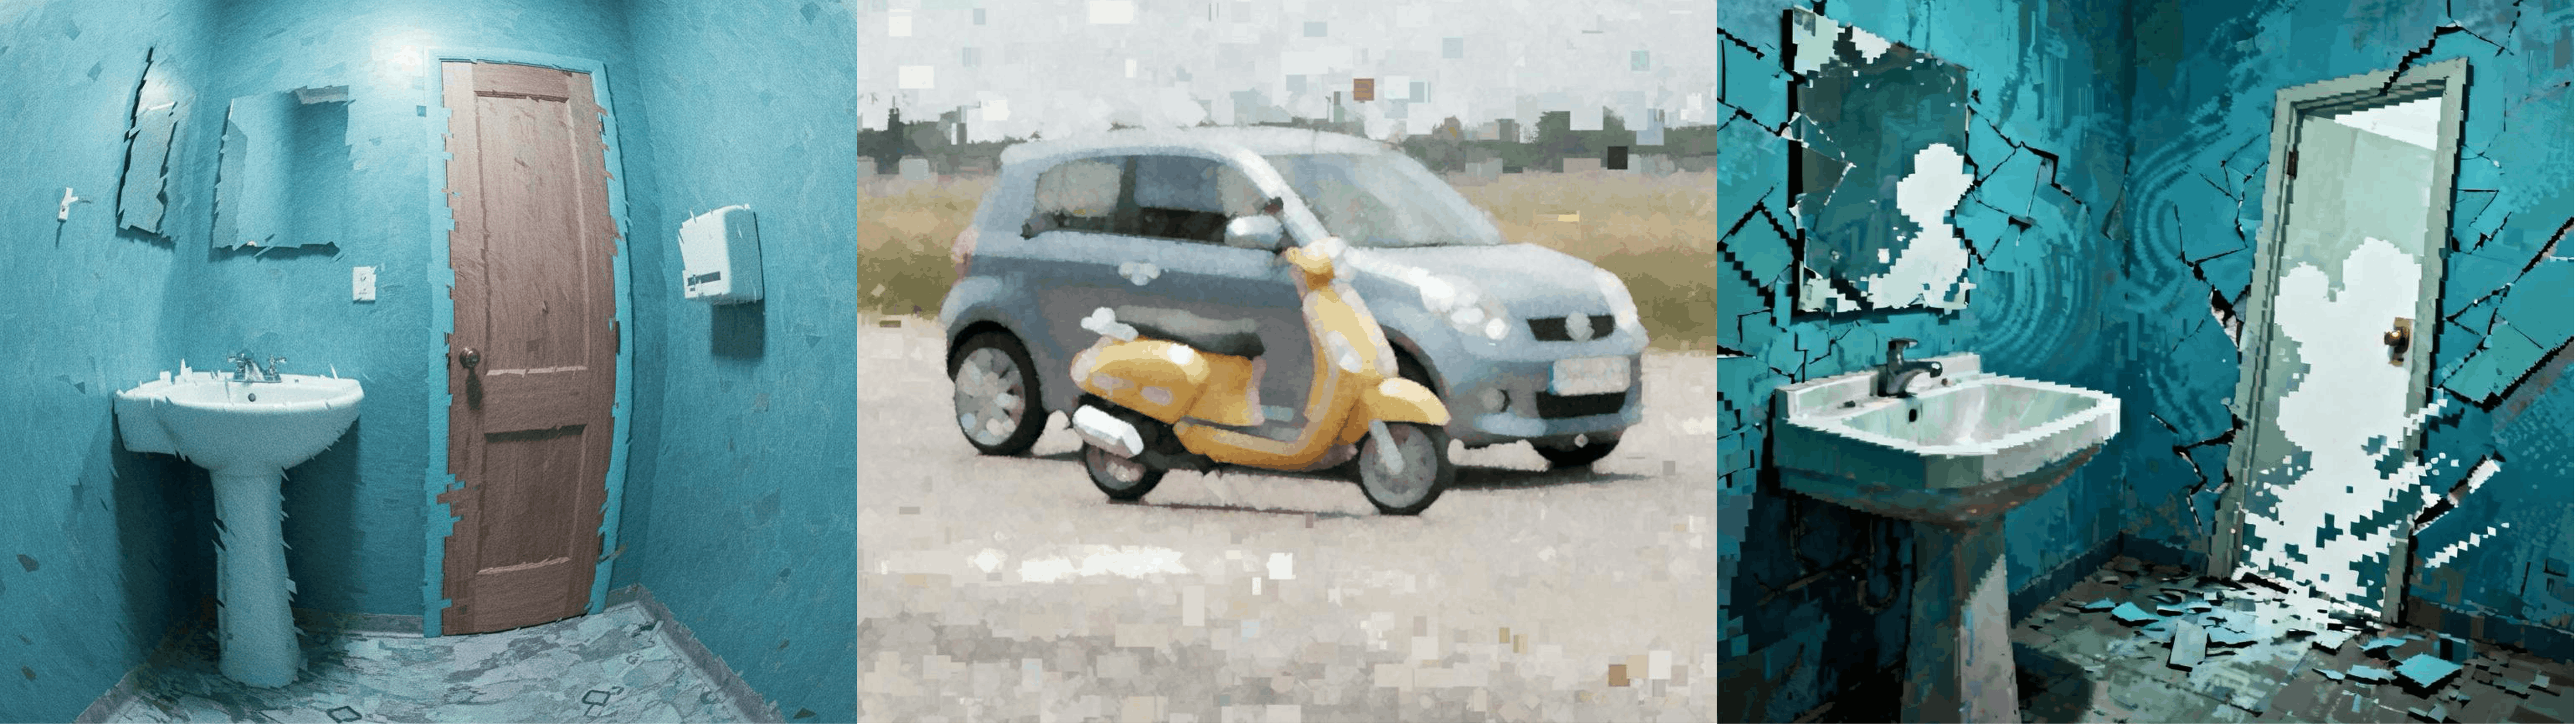
\includegraphics[width=\linewidth]{sec/imgs/demo.png}
    \caption{Successfully generated wide-spectrum aesthetics images.}
    \label{fig:placeholder}
    \vspace{-0.1in}
\end{figure}

For each image pair, an original image ($I_o$) and a wide-spectrum aesthetics image ($I_a$), we computed preference scores using a reward model ($r$) for both the original prompt ($p_o$) and the wide-spectrum aesthetics prompt ($p_a$), yielding four scores per model: $r(I_o, p_a)$, $r(I_a, p_a)$, $r(I_o, p_o)$, and $r(I_a, p_o)$. Scores with $p_o$ measure objective image quality and whether the model successfully produced wide-spectrum aesthetic content; scores with $p_a$ assess whether reward models can correctly identify such images when explicitly guided. We also computed the BLIP score for wide-spectrum aesthetic images using the same prompt, verifying that images retained the main concept while incorporating the requested modifications. We specifically measure the difference between aesthetics scores for $p_o$ and $p_a$ to avoid the case where models generated ``failed'' images consistently without the user's instructions.

\begin{table}[t]
 \centering
 \caption{Statistical Tests of How Each Aesthetics-Aligned Model Compared to Their Base Model. For p-values, a * is placed if the $p<10^{-5}$ and ** is placed if the $p<10^{-10}$.}
 \small
 \scalebox{0.8}{
\begin{tabular}{llllll}
\toprule
 & HPSv3 $p$& HPSv3 $r$& $J$ $p$& $J$ $r$&McNemar's $p$\\
\midrule
DanceFlux & ** & -0.81 & ** & -0.72 &**\\
Playground & ** & -0.59 & * & -0.35 &*\\
SD3.5M-PickScore & ** & -0.70 & ** & -0.45 &0.57\\
\bottomrule
\end{tabular}}
 \label{tab:align_p}
 \vspace{-0.2in}
\end{table}

The evaluated reward models include PickScore \cite{kirstain_pick--pic_2023}, ImageReward \cite{xu_imagereward_2023}, HPSv2.1 \cite{wu_human_2023}, MPS \cite{zhang_learning_2024}, HPSv3 \cite{ma_hpsv3_2025}, CLIP-L \cite{radford_learning_2021}, and BLIP-L \cite{li_blip_2022}. CLIP-L and BLIP-L are non-preference-aligned image-text matching models and base models for several reward models (HPSv2.1, PickScore, MPS, ImageReward), included to test whether small vision-language models can interpret complex wide-spectrum aesthetic prompts. We also collected per-dimension scores from $J$ for both $I_o$ and $I_a$ to verify whether generation models correctly followed $p_a$. For ground truth, we used \texttt{Qwen/Qwen3-VL-235B-A22B-Instruct} to judge which image in each pair better adhered to $p_a$, validated by human evaluation (details in Appendix Human Eval). The LLM and human ratings achieved a quadratic Cohen's kappa of 0.80, indicating strong agreement \cite{mchugh_interrater_2012}. We additionally used GPT-5-Chat as an external baseline to compare against Qwen's results. Note that the LLM-as-judge serves as only one metric for the generative benchmark and only a filtering stage for the reward-model benchmark.